\documentclass[12pt]{article}
\usepackage[top=2.5cm, bottom=2.5cm, left=3cm, right=3cm]{geometry}
\usepackage{graphicx}
\begin{document}


\begin{center}
\begin{normalsize}
\textbf\sl{MAKERERE 
\includegraphics[scale=0.5]{logo} UNIVERSITY }\\


\textbf\sl{FACULTY OF COMPUTING AND INFORMATICS TECHNOLOGY} \\
\textbf\sl{SCHOOL OF COMPUTING AND INFORMATICS TECHNOLOGY} \\
\textbf\sl{DEPARTMENT OF COMPUTER SCIENCE} \\
\textbf\sl{BACHELOR OF SCIENCE IN COMPUTER SCIENCE} \\
\textbf\sl{BIT 2207 RESEARCH METHODOLOGY} \\
\textbf\sl{LECTURER: ERNEST MWEBAZE} \\


\textbf{ABILA JOSHUA : 16/U/19130/PS : 216021700}\\



\end{normalsize}
\end{center}



\newpage

\begin{center}
\textsc{ILLEGAL PLAYER LICENSE ISSUING IN THE NAKAWA DIVISION UNDER THE  NATIONAL DIVISION FOOTBALL ASSOCIATION }\\


\end{center}

\section{Abstract}
\paragraph{•}
There is an alarming rampancy of clubs issuing fake player licenses ,resulting to a series of complaints from several clubs,match fixing,match forfeiting .Currently in the National division football Association 75 percent of fake player licenses  arise every season ,these issues remain painfully pending and unresolved.
\section{Introduction}
\paragraph{•}
The national division football association (NDFA) is under FUFA in uganda ,CAF in africa and FIFA globally . This association is an initiative of Fufa to promote grassroot football ,use football  as a symbol of unity throughout all regions in the country aswell as nuture young talents ,keeping track of promising young talents with great potential to reach great limits in football.This all is an effort to have a strong unit of fresh talents to blend into the National football team ,uganda cranes as time slips by .

\paragraph{•}
whilst this beautiful endeavour sprouts ,it has picked keen interest of the public stakeholders and researchers to solve the puzzling mystery of fake player licensing by clubs.
\paragraph{•}
This document describes the kind of data to be collected during research about this spreading disease at hand of clubs issuing fake licenses to players. It also includes sample data that was collected during research.

\section{Data Form}
In this research, data and information was collected by observation and interviews from spectators during national 4TH and 5TH  division football matches  .
\subsection{name }
\paragraph{•}
field where a spectator eneter his name 
\paragraph{•}

\subsection{Location of stadium}
\paragraph{•}
This field specifies where the games was hosted .
\subsection{Image of player involved }
\paragraph{•}
enables a photo shot of the player alleged to have a fake license.
\subsection{club of alleged player}
\paragraph{•}
captures data of the alleged player's club

\subsection{ Date the game was played}
\paragraph{•}
This field is to input the date a specific league is played.
.
\subsection{How the issue was resolved }
\paragraph{•}
this field enables an audio recording of the scene as its caught of glimpse by the spectator.

\subsection{assumptions why the club used an unlicensed player  }
\paragraph{•}
this is a text field that a spectator gives a reason why the club used a fake license .

\section{Sample Form}
\paragraph{•}
\textbf{spectator name  }\\
kibuuka

\paragraph{•}
\textbf{location of stadium }\\
Latitude:0.3200; Longitude:32.6575

\paragraph{•}
\textbf{name of stadium }\\
Butabika


\paragraph{•}
\textbf{image of player invovled}\\
\begin{figure}
		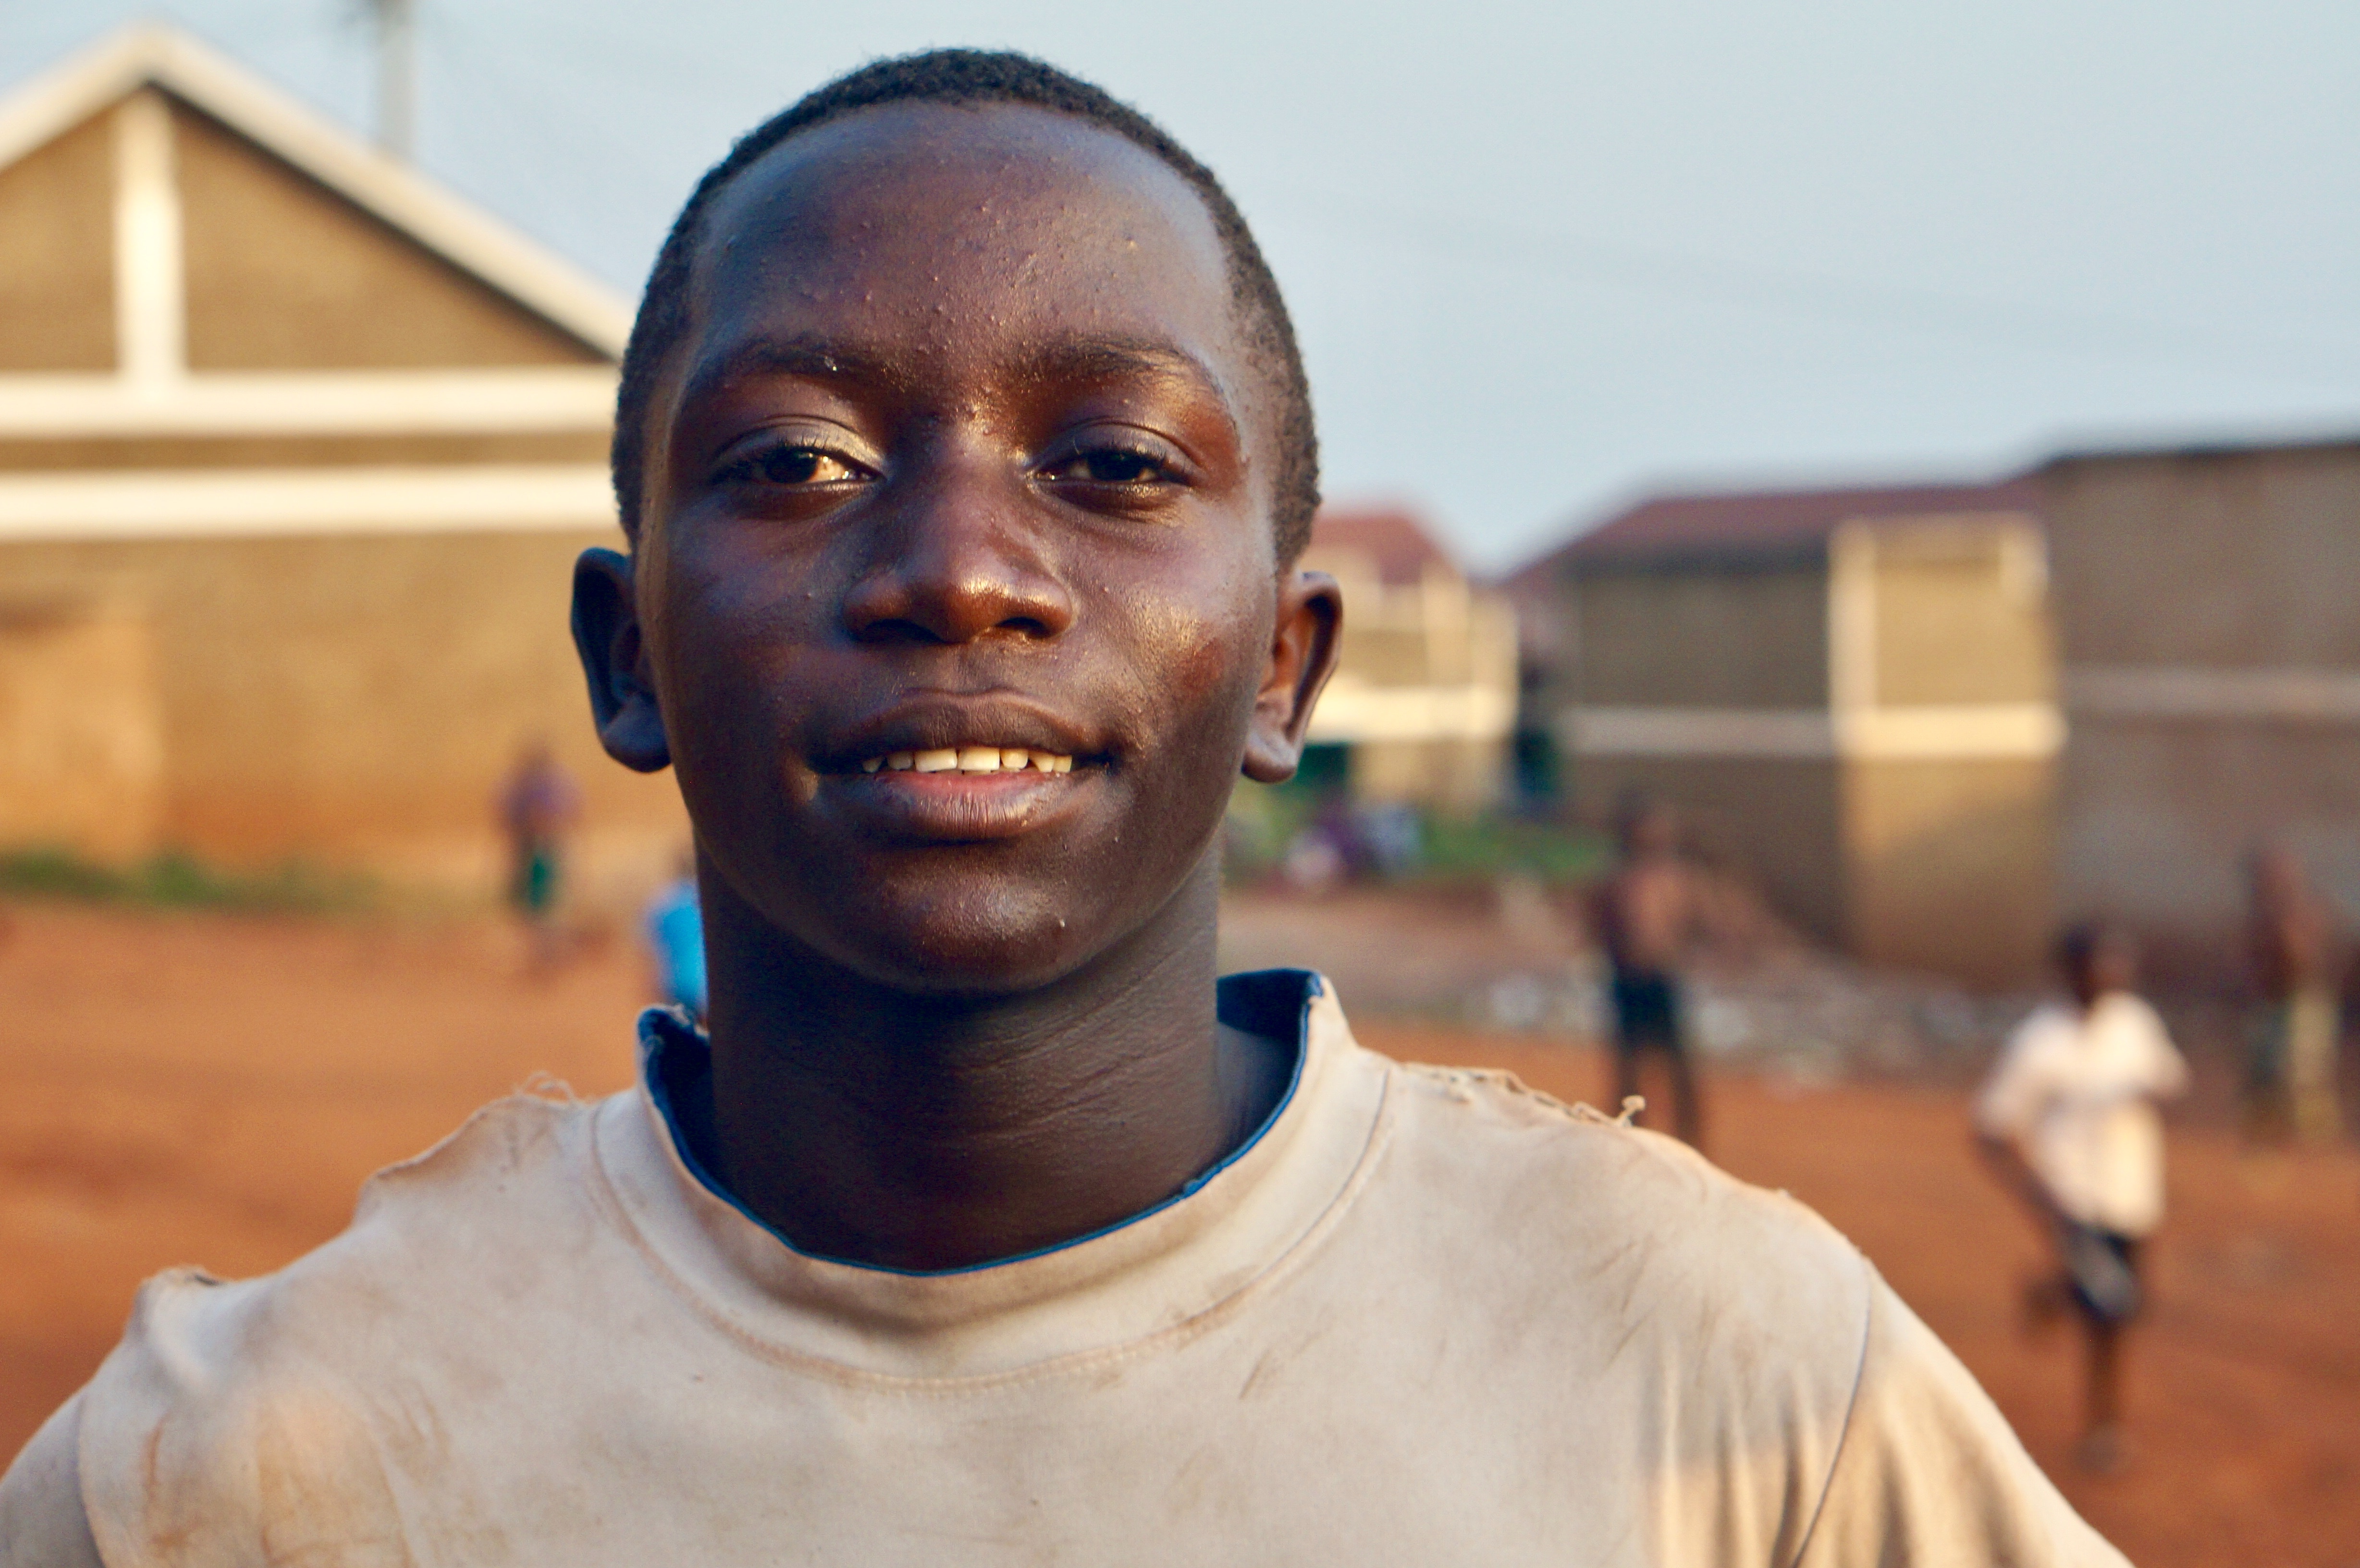
\includegraphics[scale=0.5]{odene.jpg} 
			\end{figure}


\paragraph{•}
\textbf{club of player involved}\\
Namataba rifo

\paragraph{•}
\textbf{assumptions why club used an unlicensed player}\\
afraid of relegation 

\paragraph{•}
\textbf{numberof unlicensed players}\\
1

\paragraph{•}
\textbf{date game was played}
15th/02/2017

\paragraph{•}
\textbf{How the issue was resolved}\\
player was sent off the pitch

\end{document}